\documentclass[a4paper,oneside,12pt]{article}
\usepackage[portuguese]{babel}
\usepackage{graphicx}
\usepackage{listings}
\usepackage{indentfirst}
\usepackage{fontspec}

\usepackage{xcolor}

\definecolor{codegreen}{rgb}{0,0.6,0}
\definecolor{codegray}{rgb}{0.5,0.5,0.5}
\definecolor{codepurple}{rgb}{0.58,0,0.82}
\definecolor{backcolour}{rgb}{0.95,0.95,0.92}

\lstdefinestyle{mystyle}{
    backgroundcolor=\color{backcolour},   
    commentstyle=\color{codegreen},
    keywordstyle=\color{magenta},
    numberstyle=\tiny\color{codegray},
    stringstyle=\color{codepurple},
    basicstyle=\ttfamily\footnotesize,
    breakatwhitespace=false,         
    breaklines=true,                 
    captionpos=b,                    
    keepspaces=true,                 
    numbers=left,                    
    numbersep=5pt,                  
    showspaces=false,                
    showstringspaces=false,
    showtabs=false,                  
    tabsize=2
}

\newcommand{\mybox}[1]{
    \colorbox{backcolour}{\textbf{#1}}
}

\lstset{style=mystyle}

\linespread{1.5}
\setmainfont{Times New Roman}

\title{Usando MoonScript com LÖVE}
\author{Canoi Gomes}
\date{25 de Fevereiro de 2017}

\begin{document}

\maketitle
\newpage

\tableofcontents
\newpage

\section{Introdução}

Nesse tutorial, pretendo abordar um pouco sobre como usar o MoonScript, que é basicamente uma linguagem que é \textbf{transpilada} para Lua, com a framework LÖVE.

\begin{figure}[h]
    \centering
    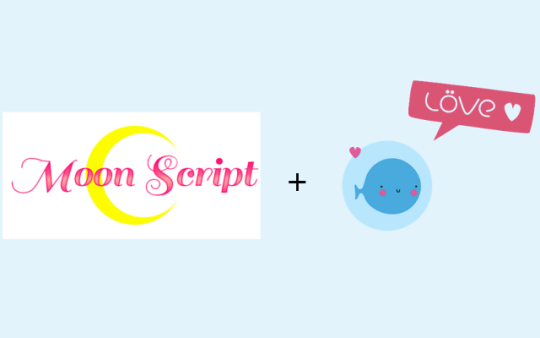
\includegraphics[width=\linewidth]{media/moonscript_with_love.png}
\end{figure}

Mas qual a vantagem de usar uma terceira linguagem ao invés de usar somente Lua direto, se no fim tudo será convertido para ela mesmo? De fato, o uso de MoonScript se dá mais por alguns recursos que a linguagem implementa onde se fossemos fazer puramente em Lua seria necessário um trabalho a mais ou (o mais indicado) usar um biblioteca externa. Alguns exemplos como Classes, os famigerados \mybox{+=} ou \mybox{-=}.

\subsection{Instalando o MoonScript}

Aqui não vou me aprofundar muito nisso, mas você pode acessar o site do MoonScript para fazer o setup no seu sistema operacional. No fim você terá basicamente dois executáveis, um \textbf{moon} para rodar os códigos MoonScript, e um \textbf{moonc} responsável por compilar o código para Lua. E pra rodar é bem simples, só chamar no terminal:

\begin{lstlisting}
moonc main.moon
\end{lstlisting}

\section{Criando Nosso main.moon}

Bom, vamos começar criando um arquivo \textbf{main.moon}, que seria relativo ao main.lua esperado pelo LÖVE. Aqui você vai escrever as funções esperadas pela LÖVE (load, update e draw), porém usando a sintaxe do MoonScript.

\begin{lstlisting}[language={[5.2]Lua}]
love.load = ->
love.update = (dt) ->
love.draw = ->
\end{lstlisting}

Fácil, né? Agora roda aquele comando anterior, o moonc, para compilar nosso código. Já adiantando um pouco aqui, você também pode rodar o comando com \mybox{moonc *.moon} e ele compila todos o .moon no diretório atual.

Mas é isso, não tem muito mistério. Porém agora gostaria de mostrar um pouco de uma aplicação prática.

\section{Criando uma Aplicação Prática}

Então vamos brincar um pouco com os recursos do MoonScript pra fazer algo legal. Vamos criar uma classe \mybox{GameObject}:

\begin{lstlisting}
class GameObject
    x: 0
    y: 0
    width: 32
    height: 32
    update: (dt) =>
    draw: () =>
\end{lstlisting}

Vamos criar tudo no main.moon mesmo, é o suficiente para esse exemplo. Bom, perceba aqui que que criei uma classe com algumas propriedades, um coisa a se atentar é que caso um desses atributos seja uma tabela, você vai precisar criar um construtor. Aqui é necessário isso devido a maneira como as tabelas se comportam dentro do Lua, que seria como ponteiros em C, então diferente de um atributo de number ou string onde os seus dados são copiados, em uma tabela somente sua referência é passada adiante.

Por exemplo:

\begin{lstlisting}
class Teste
    attributes: {}
    add_value: (value) =>
        table.insert @attributes, value

obj0 = Teste!
obj1 = Teste!

print obj0.attributes[1] -- irá printar nil
print obj1.attributes[1] -- irá printar nil também

obj0\add_value 1 -- adiciona o valor 1 à tabela

print obj0.attributes[1] -- irá printar 1
print obj1.attributes[1] -- irá printar 1 também

obj3 = Teste!
print obj3.attributes[1] -- também irá printar 1
\end{lstlisting}

Note que como a referência é passada adiante, então os dados da tabela serão compartilhado por todas as instâncias da classe. Com certeza você irá querer fazer isso em alguns casos, mas caso contrário, nós podemos utilizar um recurso das próprias classes do MoonScript, que são os construtores. Para isso é só definirmos uma função \mybox{new} dentro da nossa classe.

\begin{lstlisting}
class Teste
    attributes: {}
    new: =>
      @attributes = {}
    add_value: (value) =>
      table.insert @attributes, value
      
obj0 = Teste!
obj1 = Teste!

print obj0.attributes[1] -- irá printar nil
print obj1.attributes[1] -- irá printar nil também

obj0\add_value 1 -- adiciona o valor 1 à tabela do obj0
  
print obj0.attributes[1] -- irá printar 1
print obj1.attributes[1] -- aqui irá printar nil
\end{lstlisting}

Voltando para o exemplo anterior, vamos extender nossa classe de GameObject para criar uma classe para o Player.

\begin{lstlisting}
class Player extends GameObject
    update: (dt) =>
        if love.keyboard.isDown "left"
            @x -= 200 * dt
        if love.keyboard.isDown "right"
            @x += 200 * dt
    draw: () =>
        love.graphics.rectangle "line", @x, @y, @width, @height
\end{lstlisting}

Aqui não tem muito mistério, criei a classe Player que é filho de GameObject, e implemento algumas funções dentro dela para update e draw. Agora é só criar uma instância da classe e então chamar seus métodos dentro das funções da LÖVE.

\begin{lstlisting}
player = Player!

love.load = ->
love.update = (dt) ->
    player\update dt
love.draw = ->
    player\draw!
\end{lstlisting}

\section{Considerações}

Algumas outras coisas interessantes de fazer é executar o comando moonc no modo espectador. Ele vai ficar checando constantemente se houve alguma mudança no arquivo, e caso tenha, irá compilá-lo. Isso pode ser feito usando a opção \textbf{-w}:

\begin{lstlisting}
moonc -w main.moon
\end{lstlisting}

Outra opção interessante é a \textbf{-t}, onde você pode definir o caminho para onde os arquivos compilados serão jogados. Acho bacana essa estrutura para usar no seu projeto:

\begin{lstlisting}
game/
    assets/
    ~lua code~
src/
    ~moon code~
\end{lstlisting}

E daí só executar:

\begin{lstlisting}
moonc -t game/ -w src/
\end{lstlisting}

E com isso todo o conteúdo necessário para rodar seu projeto estará em game/, é só empacotar tudo e distribuir.

\end{document}